\documentclass[soumission]{ir}

\titre{Initiation à la recherche \\Classification de musique non supervisée}

\auteur{Lafille Julien et Ouali Kouceilal}

\titrecourt{Classification de musique non supervisée}

\nomcourt{J. Lafille et K. Oualil}

\encadrant{Alexendre Blansché}

\motcle{Annalyse de signal, Musique, Classification, Non supervisé}

\begin{document}

\section{Introduction}

\section{Etat de l'art}
La musique étant massivement présente en format numérique, et le besoin de classer les différentes musiques
 étant toujours aussi présent, les chercheurs ont développé différentes techniques permettant d’automatiser 
 le processus.

\subsection{L’analyse et la classification musicale}
\paragraph{}
La recommandation de musique s’appuie essentiellement sur l’identification des genres. L’humain étant capable 
de reconnaître un genre musical dans 70\% des cas au bout de 3 secondes d’écoutes seulement, et dans 50\% 
des cas au bout de 0.25 secondes \cite{TechniqueSimilarites}, les chercheurs ont essayé de réaliser cette 
discrimination de manière automatique et se sont reposés sur l’analyse et l’extraction des données physiques 
des fichiers audio. Ainsi, les critères formels pris en compte ont été utilisés pour différencier les divers 
genres musicaux et attribuer chaque titre à l’un de ces genres.
\paragraph{}
La difficulté réside dans le choix de critères pertinents, divers techniques se sont développées au fil du 
temps et les chercheurs se sont notamment basés sur la structure rythmique, la superposition des instruments, 
ou encore le timbre. Deux approches sont particulièrement utilisées dans le domaine, la première se repose 
sur l’analyse du signal, qui utilise la reconnaissance de motifs et la construction d’une “surface musicale” 
\cite{TechniqueSimilarites} et la seconde sur l'analyse des caractéristiques physiques de haut niveau se 
basant sur l’analyse de partitions musicales (qui permet d’extraire des données telle que la hauteur d’une 
note), cette dernière technique étant possible même quand le fichier audio n’est pas disponible.

\subsection{Les systèmes de recommandation}
\paragraph{}
Souvent dans le but de fidéliser l’utilisateur et maximiser le temps qu’il passe sur la plateforme, les 
systèmes de recommandation (que ce soit celles utilisées par les plateformes de streaming audio comme Deezer 
et Spotify, vidéo comme Youtube et les réseaux sociaux comme Facebook) utilisent les données récoltées au 
cours de l’utilisation du service par un profil utilisateur pour affiner les recommandations en plus des 
autres techniques de classements.

\paragraph{}
Une analyse contextuelle est bien souvent nécessaire pour avoir des résultats plus proches de la sensibilité 
humaine, en prenant en compte les subjectivités liées à la reconnaissance de genres par l’Homme (comme les 
influences culturelles ou l’émotion). Cette analyse se fait souvent sur les métadonnées récoltées en continu 
et qui évoluent en suivant les tendances. Pour cela, ils se basent sur l’utilisateur en lui-même et ses 
interactions (autant avec les items qu’avec les autres utilisateurs). On utilise les deux approches, souvent 
complémentaires, qui sont : 
\begin{itemize}
    \item{Le filtrage par contenu, s'intéressant au couple \textit{[Profil utilisateur-Item]} et sur l’appréciation 
    de l’utilisateur concernant cet item. La proximité des items est affinée en recueillant ces appréciations 
    et l’utilisateur se voit recommander les items les plus pertinents en vue de sa notation ou de son 
    nombre de consultations des items voisins.}
    \\
    \item{Le filtrage collaboratif, quant à lui, crée une proximité sociale entre les utilisateurs et classe 
    les items selon les affinités entre utilisateurs afin de proposer un item “populaire” au sein d’un 
    groupe aux utilisateurs en faisant partie.}
\end{itemize}

\paragraph{}
Mais c’est généralement des méthodes hybrides qui sont utilisées dans les services de recommandation. Ces 
données sont exploitées par des algorithmes de classification supervisés en se reposant sur les classements 
faits par les libraires, les radios et les musicologues pour les caractéristiques liées aux musiques et sur 
les données récoltées lors de l’utilisation du service par l’utilisateur pour ce qui est des métadonnées. 
Mais les différentes subjectivités et les définitions parfois très vagues de certains genres sont une source 
importante d’erreurs. De plus, l’analyse contextuelle favorise l’enfermement de l’auditeur dans un univers 
restreint et peine à réellement recommander de nouveaux genres, s’ajoute à cela qu’en prenant en compte la 
popularité des morceaux, en cas de filtrage collaboratif, il est moins probable que ces techniques 
recommandent un titre impopulaire mais proche des goûts musicaux de l’auditeur (qu’il serait donc 
susceptible d'apprécier).

\subsection{Propositions}
\paragraph{}
Les techniques énoncées précédemments se basent sur un mimétisme des choix des utilisateurs et sur les 
étiquetages et ne se reposent pas sur une classification objective de la musique. De ce fait, il est plus 
difficile de classifier les genres de manière universelle. Nous nous proposons donc de chercher un moyen de 
classer la musique de façon plus indépendante de l’utilisateur dans un premier temps, mais aussi de façon 
indépendante des genre déjà définis, et ce pour plusieurs raisons :
\begin{itemize}
    \item {Il n’y a pas de réel consensus sur une liste exhaustive de genres musicaux.}
    \item {La définition de certains genres musicaux étant floue et assez vague pour comprendre une même 
    chanson dans plusieurs genres.}
    \item {Ils sont basés sur des influences culturelles et parfois ancrées dans un air temporel défini.}
\end{itemize}

\paragraph{}
Une fois que le classement ait été établi grâce à des algorithmes de classification non supervisée (qui se 
baseront donc essentiellement sur l’analyse musicale), nous intégrerons les préférences de l’auditeur au 
modèle pour isoler et pouvoir proposer les items les plus proches de ses envies. Cette classification 
indépendante des constructions “artificielles” de catégories de musiques est susceptible de rassembler les 
items dans des groupes aux frontières potentiellement mieux définies.

\section{Analyse audio}
\paragraph{}
Les algorithmes de clustering ont besoin de données pour effectuer une classification. Nos données initiales 
sont des fichiers audio, ils contiennent le signal musical en lui-même et quelques métadonnées telles que le 
titre, l’artiste ou encore l'album. Nous voulions dans notre démarche proposer des chansons similaires sans 
se baser sur les métadonnées des chansons, mais plutôt la similitude des chansons. La seule métadonnée que 
nous utiliserons est donc la durée.

\paragraph{}
Il n’est pas possible de donner aux algorithmes de clustering directement le signal, nous devons donc 
“simplifier” le signal en données exploitables pour ces algorithmes. Beaucoup de travaux ont été réalisés 
en analyse de musique et analyse vocale. Un grand nombre de ces travaux se base sur l’analyse du signal 
audio. Certains critères calculables à partir du signal sont assez récurrents dans les différents travaux 
du domaine, c’est pourquoi nous avons décidé de les utiliser comme critères pour effectuer notre 
classification.

\subsection{Présentation des données}
\paragraph{}
Nous avons retenu 4 critères assez communs en analyse audio que nous allons détailler dans cette section : 
le Zero Crossing Rate, le Root Mean Square, la Centroid et le Spread. Nous devons déjà expliquer la nature 
de nos données.

\paragraph{}
Un signal audio analogique peut être vu comme la pression exercée par une source sur l’air qui l’entoure 
dans le temps. Cette pression de l’air est captée par nos oreilles ou bien un microphone. Sa nature est 
continue, pour transformer ce signal continu en information on utiliser une méthode d'échantillonnage pour 
discrétiser l’information, on a alors un signal numérique.

\begin{figure}[ht]
    \centering
    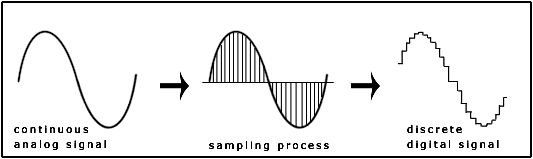
\includegraphics[scale=0.7]{images/Sampling-of-audio-signal.png}
    \caption{Echantillonage d'un signal continu}
    \label{ex_echantillonage}
\end{figure}

\paragraph{}
La fréquence d'échantillonnage (Fe) détermine la fréquence à laquelle chaque échantillon est pris. Plus la 
fréquence est haute plus le signal numérique est proche du signal analogique. Le sampling mène à une  perte 
d’information s’il existe des variations plus rapides que la fréquence d'échantillonnage. De manière 
générale on dit que le signal est bien représenté tant qu’il ne contient pas une fréquence supérieure à 
$\frac{Fe}{2}$. C’est pourquoi le standard dans l’industrie de la musique est \textit{Fe = 44100 Hz} ce qui 
permet de couvrir tout le spectre de l’audition humaine ( 20 Hz à 20000 Hz) avec un peu de marge.

\paragraph{}
Une chanson contient en général deux pistes audio pour donner un effet stéréo. Nous convertissons ces deux pistes 
stéréo en une seule piste mono pour conduire nos analyses. Nous découpons ensuite le signal en morceaux plus
 courts pour calculer chacun de nos critères en gardant l’aspect temporel de la musique. Nous avons choisit 
 de découper le signal en sections de une seconde, qui est un bon compromis entre vitesses de calcul des 
 critères et précision temporelle \cite{Survey}.

\subsection{Critères temporels}
\paragraph{}
Nous pouvons maintenant calculer deux de nos critères, le premier étant le zero crossing rate, ou taux de 
passage par zéro. Ce critère permet d’avoir une estimation du timbre du signal (un signal aigu passera par 
zéro plus fréquemment qu’un signal grave).
\begin{equation}
    ZCR = \frac{1}{N}*\sum_{n = 1}^{N} \delta( x_{n-1}.x_n \leqslant 0 )
\end{equation}

\noindent{Avec $x_i$ le i-ème echantillon du signal, $N$ le nombre d'échantillons et : }\\

$\delta(x)=\begin{cases}
    1, & \text{si $x$ est vrai}.\\
    0, & \text{sinon}.
\end{cases}$

\paragraph{}
Le second critère est le root mean square : ce critère permet de calculer l'énergie moyenne du signal sur 
une période.
\begin{equation}
    RMS = \sqrt{\frac{1}{N}.\sum_{n = 0}^{N-1} x_n^2}
\end{equation}

\subsection{Critères fréquentiels}
Nos deux autres critères s’intéressent à l’aspect fréquentiel d’un signal.Tout signal peut être décomposé 
comme une somme de fonctions sinusoïdales avec différentes fréquences. La transformation de Fourier est un 
outil nous permettant d’effectuer un passage du domaine temporel au domaine fréquentiel. Dans le domaine 
temporel on observe l’intensité du signal à un moment donné. Dans le domaine fréquentiel on observe 
l’intensité d’une fréquence sur la totalité du signal. L’intensité de la  k-ième fréquence d’un signal s à N 
échantillons est donnée par :

\begin{equation}
    s_k = \sum_{n = 0}^{N-1} x_n.e^{-2 i \pi k. \frac{n}{N}}
    \qquad\text{pour $0 \leqslant k < N$}
\end{equation}

ou la k-ième fréquence vaut : $-\frac{Fe}{2} (\frac{2k}{N} - 1)$

\paragraph{}
Les intensités obtenues sont donc des nombres complexes. Pour nos analyses on pourra utiliser $|s_k|$. La 
moitié de ces intensités représente des fréquences négatives. Dans le cas d'un signal réel comme le notre 
il existe une symétrie parfaite entre les fréquences négatives et positives. Il est important de conserver 
les fréquences négatives pour effectuer la transformée inverse, mais pour analyser le signal nous pouvons 
nous permettre de les ignorer. Nous considérons donc les fréquences dans la plage 0 à $\frac{Fe}{2}$ Hz.

\begin{figure}[ht]
    \centering
    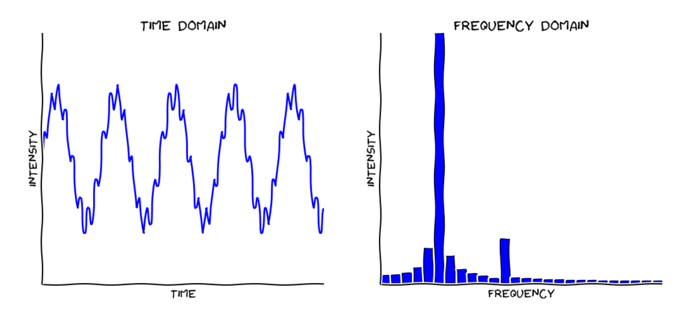
\includegraphics[scale=0.7]{images/Fourier.png}
    \caption{Passage du domaine temporel au domaine fréquenciel}
    \label{ex_Fourier}
\end{figure}

\paragraph{}
Nous pouvons ainsi calculer nos deux derniers critères, à commencer par la Spectral Centroid : Elle représente la 
fréquence moyenne du signal sur la période analysée.

\begin{equation}
    Centroid = \frac{ \sum_{k = 0}^{T-1} \frac{Fe}{2} \frac{k}{T} * s_k}{\sum_{k=0}^{T-1} s_k}
    \qquad \textit{avec T le nombre de fréquences}
\end{equation}

Le dernier critère que nous calculons est le Spectral Spread. Ce critère représente l'écart de fréquence du
signal sur la période analysée.

\begin{equation}
    Spread = \frac{ \sum_{k = 0}^{T-1} \frac{Fe}{2} \frac{k}{T} (s_k - Centroid)^2}{\sum_{k=0}^{T-1} s_k}
    \qquad \textit{avec T le nombre de fréquences}
\end{equation}

Ces calculs sont réalisés par un programme que nous avons écrit dans le language C\#. Ces calculs nous donnent 
donc quatre vecteurs d’une longueur égale à la durée de la chanson en seconde. Nous utiliserons ces données 
pour effectuer notre clustering par la suite.

\section{Classification}
Notre but étant d’obtenir une classification “naturelle” des chansons, et d’obtenir un ensemble d’univers 
musicaux cohérents. Nous utilisons donc des algorithmes de classifications non supervisées avec les données 
recueillies précédemment. Nous considérons pour chaque chanson la médiane et l’écart type de chaque critère
ainsi que sa durée.

\subsection{Méthodes adoptées}
Nous avons testé 4 algorithmes de clustering pour classifier les différents genres musicaux avec, en entrée 
les 9 valeurs extraites des différentes analyses :
\begin{itemize}
    \item{\textbf{K-Means} : divise les items en un nombre défini de clusters de variances égales et minimisant le 
    critère de la somme des carrés au sein d’un cluster}
    \item {\textbf{Agglomerative Clustering} : Algorithme de classification hiérarchique à approche ascendante. 
    Pouvant s’utiliser avec plusieurs critères de liaison : simple, moyenne, complète, ward, c’est ce dernier 
    que nous avons choisi et qui est assez proche de la fonction objectif de K-Means mais abordée avec une 
    approche hiérarchique agglomérative.}
    \item{\textbf{Affinity Propagation} : classifie les données en considérant successivement les paires d’items jusqu’à 
    convergence pour décider, ensuite, d’un ensemble de données “représentatifs”. Cet algorithme ayant la 
    particularité de choisir lui-même le nombre de clusters pour les données fournies, nous nous sommes basés 
    sur ses résultats pour décider du nombre de clusters pour les autres algorithmes testés.}
    \item{\textbf{Spectral Clustering} : Classifie les items en suivant l’imbrication de la matrice d’affinité entre 
    échantillons, suivie d’un K-Mean dans l’espace dimensionnel faible.}
\end{itemize}

\subsection{Mise en oeuvre}
Pour mettre en oeuvre ces algorithmes, nous avons développé un programme en Python et utilisons une bibliothèque 
libre d’apprentissage automatique : Scikit-learn. La communication avec le programme d’analyse se fait via un 
fichier JSON. Nous obtenons les résultats suivants :

\begin{figure}[ht]
    \centering

    \caption{Clusters formés par K-means avec et sans PCA.}
    \label{clsuter_kmeans}
\end{figure}

\begin{figure}[ht]
    \centering

    \caption{Clusters formés par Agglomerative Clustering avec et sans PCA.}
    \label{clsuter_agglo}
\end{figure}

\begin{figure}[ht]
    \centering

    \caption{Clusters formés par Affinity Propagation avec et sans PCA.}
    \label{clsuter_affinity}
\end{figure}

\begin{figure}[ht]
    \centering

    \caption{Clusters formés par Spectral Clustering avec et sans PCA.}
    \label{clsuter_spectral}
\end{figure}

Les données présentent, à gauche, une représentation en 2D des clusters obtenus en appliquant les algorithmes 
sur les 9 données recueillies, et à droite, la régression des données après application de l’algorithme PCA 
(Principal Component Analysis).On peut constater une forte similarité entre les clusters des différents 
algorithmes, en particulier sans utilisation de PCA. Avec la réduction des données, les résultats sont assez 
proches pour chacun de K-Means, Agglomerative Clustering et Affinity Propagation, avec quelques différences pour
 les données les plus excentrées. En revanche, la classification se fait de manière différente pour Spectral 
 Clustering (algorithme traditionnellement utilisé sur un faible nombre de clusters). Nous pouvons, ici, 
 remarquer un grand nombre de clusters contenant peu d’items, au niveau de ce qui semble être le centre de 
 gravité du jeu de données, englobés par un cluster beaucoup plus imposant suivi des autres clusters tout autour.

\section{Résultat expérimentaux}
Après avoir extrait les données et appliqué les algorithmes de classification non supervisés sur 675 chansons et musiques tirées 
d’univers musicaux variés allant de While My Guitar Gently Weeps des Beatles à Ride the Lightning de Metallica 
en passant par Diriyi de Ait Menguellet. Nous nous proposons de tester l’efficacité de la classification obtenue.

\subsection{Protocole}
L’évaluation s’est faite sur la classifiant les items avec une réduction des données grâce à PCA puis sans. Les 
tests, réalisés sur un échantillon de 5 personnes, consistaient à tirer aléatoirement 3 morceaux d’un même 
cluster et les faire écouter aux participants. Ensuite, chaque participant propose une chanson qu’il juge proche 
des morceaux écoutés, et une chanson qu’il juge, au contraire, de styles différent. Nous renouvelons l’expérience 
de chaque participant avec chaque algorithme de clustering testé.Une fois ces données recueillies, nous 
appliquons notre programme d’analyse sur les chansons proposées et demandons à l’algorithme correspondant à la 
réponse de prédire la classe du nouvel item afin de comparer avec les réponses des participants.

\subsection{Resultats}
\paragraph{}
Nous avons, tout d’abord, testé nos algorithmes sans réduction des données (donc sur 9 dimensions) avons testé 
la prédiction des chansons proposées par les participants aux tests et les avons comparé à leur appréciation. Le 
taux de prédictions correctes pour les chansons de style jugés proches est, globalement, de 35\% et pour les 
chansons de style jugés différent est de 100\%.


\begin{figure}[ht]
    \centering
    \begin{tabular}{ccccc}
        \phantom & K-means & Agglomerative & Affinity & Spectral\\
        \hline
        réussite : chansons proches & 20\%& 20\% & 20\% & 80\%\\
        réussite : chansons différentes & 100\% & 100\% & 100\% & 100\%\\
        \hline
    \end{tabular}
    \caption{Taux de réussite des algorythmes sans PCA.}
    \label{test}
\end{figure}

\paragraph{}
Ensuite, nous avons réalisé le même test avec le même échantillon de 5 personnes avec les résultats des 
classification après réduction des données (en utilisant l’algorithme PCA). Cette fois-ci le taux de prédictions 
correctes pour les chansons de style jugés proches est de 55\% et pour les chansons de style jugés différent, il 
est de 100\%.

\begin{figure}[ht]
    \centering
    \begin{tabular}{ccccc}
        \phantom & K-means & Agglomerative & Affinity & Spectral\\
        \hline
        réussite : chansons proches & 60\%& 60\% & 60\% & 40\%\\
        réussite : chansons différentes & 100\% & 100\% & 100\% & 100\%\\
        \hline
    \end{tabular}
    \caption{Taux de réussite des algorythmes avec PCA.}
    \label{test_pca}
\end{figure}

\paragraph{}
Les résultats nous montrent que la prédiction de non-appartenance d’une chanson à un cluster jugé différent d’elle
est tout le temps correct. Les méthodes que nous avons utilisées semblent discriminer correctement les genres très 
différents, indépendamment de l’algorithme de classification ou de l’application ou non de PCA. En ce qui 
concerne l'efficacité de la prédiction positive (l’item appartient à la classe), il est globalement plus 
intéressant d’utiliser une réduction PCA , correcte dans 55\% des cas, avec K-Means, Agglomerative Clustering et 
Affinity Propagation qui présentent des taux de prédiction corrects de 60\% chacun (contre 20\% chacun si les 
données ne sont pas réduites). En revanche, on peut remarquer que l’algorithme Spectral Clustering est le plus 
performant avec 80\% de taux de prédictions positives correctes quand il est utilisé sans réduction des données. 
Mais tous les résultats de ces tests sont à prendre avec prudence du fait du faible nombre d'échantillons de 
l’expérience.

\paragraph{}
La classification de la musique grâce à des algorithmes de clustering semble possible. La faible efficacité de 
certains algorithmes peut s’expliquer de deux manières différentes. Premièrement, le faible nombre de données 
(675 chansons classifiées) peut affecter significativement les résultats potentiels et ces algorithmes pourraient 
affiner leur classification avec un jeu de données plus conséquent. Deuxièmement la réduction des données à une 
simple médiane et écart-type alors que les valeurs peuvent être très différentes à divers moments de la musique 
(pour rappel, 4 valeurs sont calculées en étudiant le signal de chaque fichier audio divisé en fenêtres de 1 
seconde).

\section{Conclusion}
Le travail mené au cours de cette étude a permis d’obtenir un système de classement des genres musicaux basé sur 
des algorithmes de classification non supervisés. Afin de produire un ensemble de critères efficaces, nous avons 
expérimenté divers descripteurs et avons retenu les plus pertinents et ceux dont les résultats sont les plus 
significatifs.  Les données récoltées après les analyses des fichiers audio ont pu servir à la classification des 
différents morceaux, et comme nous avons pu nous y attendre, créé des genres assez différents de ceux que l’on 
pourrait imaginer de prime abord. Même si les principaux styles musicaux semblent être représentés, certains 
clusters contiennent des chansons que l’on aurait pu imaginer plus différentes. La classification résultant de 
notre travail peut servir à étiqueter les chansons de manière plus objective, et peut permettre une 
recommandation plus basée sur la musique aux auditeurs et moins sur les statistiques d’écoute de cette musique, 
notamment la popularité de la chanson ou de l’artiste, l’effet de mode qui fait que l’on peut être influencé par 
l’évolution des gout du groupe social auquel on s’identifie, ce qui permet de donner autant de chances pour des 
artistes moins connus mais dont la musique pourrait s’avérer compatible avec les goûts de l’auditeur.

\bibliographystyle{apalike}
\bibliography{IR_biblio}

\appendix

\end{document}
